\subsection{MNIST Data Set and Feature Selection}

We applied a perceptron model to classification of handwritten digits. MNIST is a standard data set with $28\times28$ pixel images of handwritten digits.
We selected the digits $0$ and $7$ and 500 training images for each class for our classification task, as they are reasonably diffenrent. To chose the right feature we plotted all regionprops in a scatter plot matrix,see figure \ref{perceptron:features} and selected solodity and eccentricity. To compare the batch and online version we used an equivalent number of maximal iterations. This means we took used the size of a batch times the maximum number of iterations in the batch case as the maximum number of iterations for the online algorithm. In our case we took $500000$ and $500$.

\begin{figure}
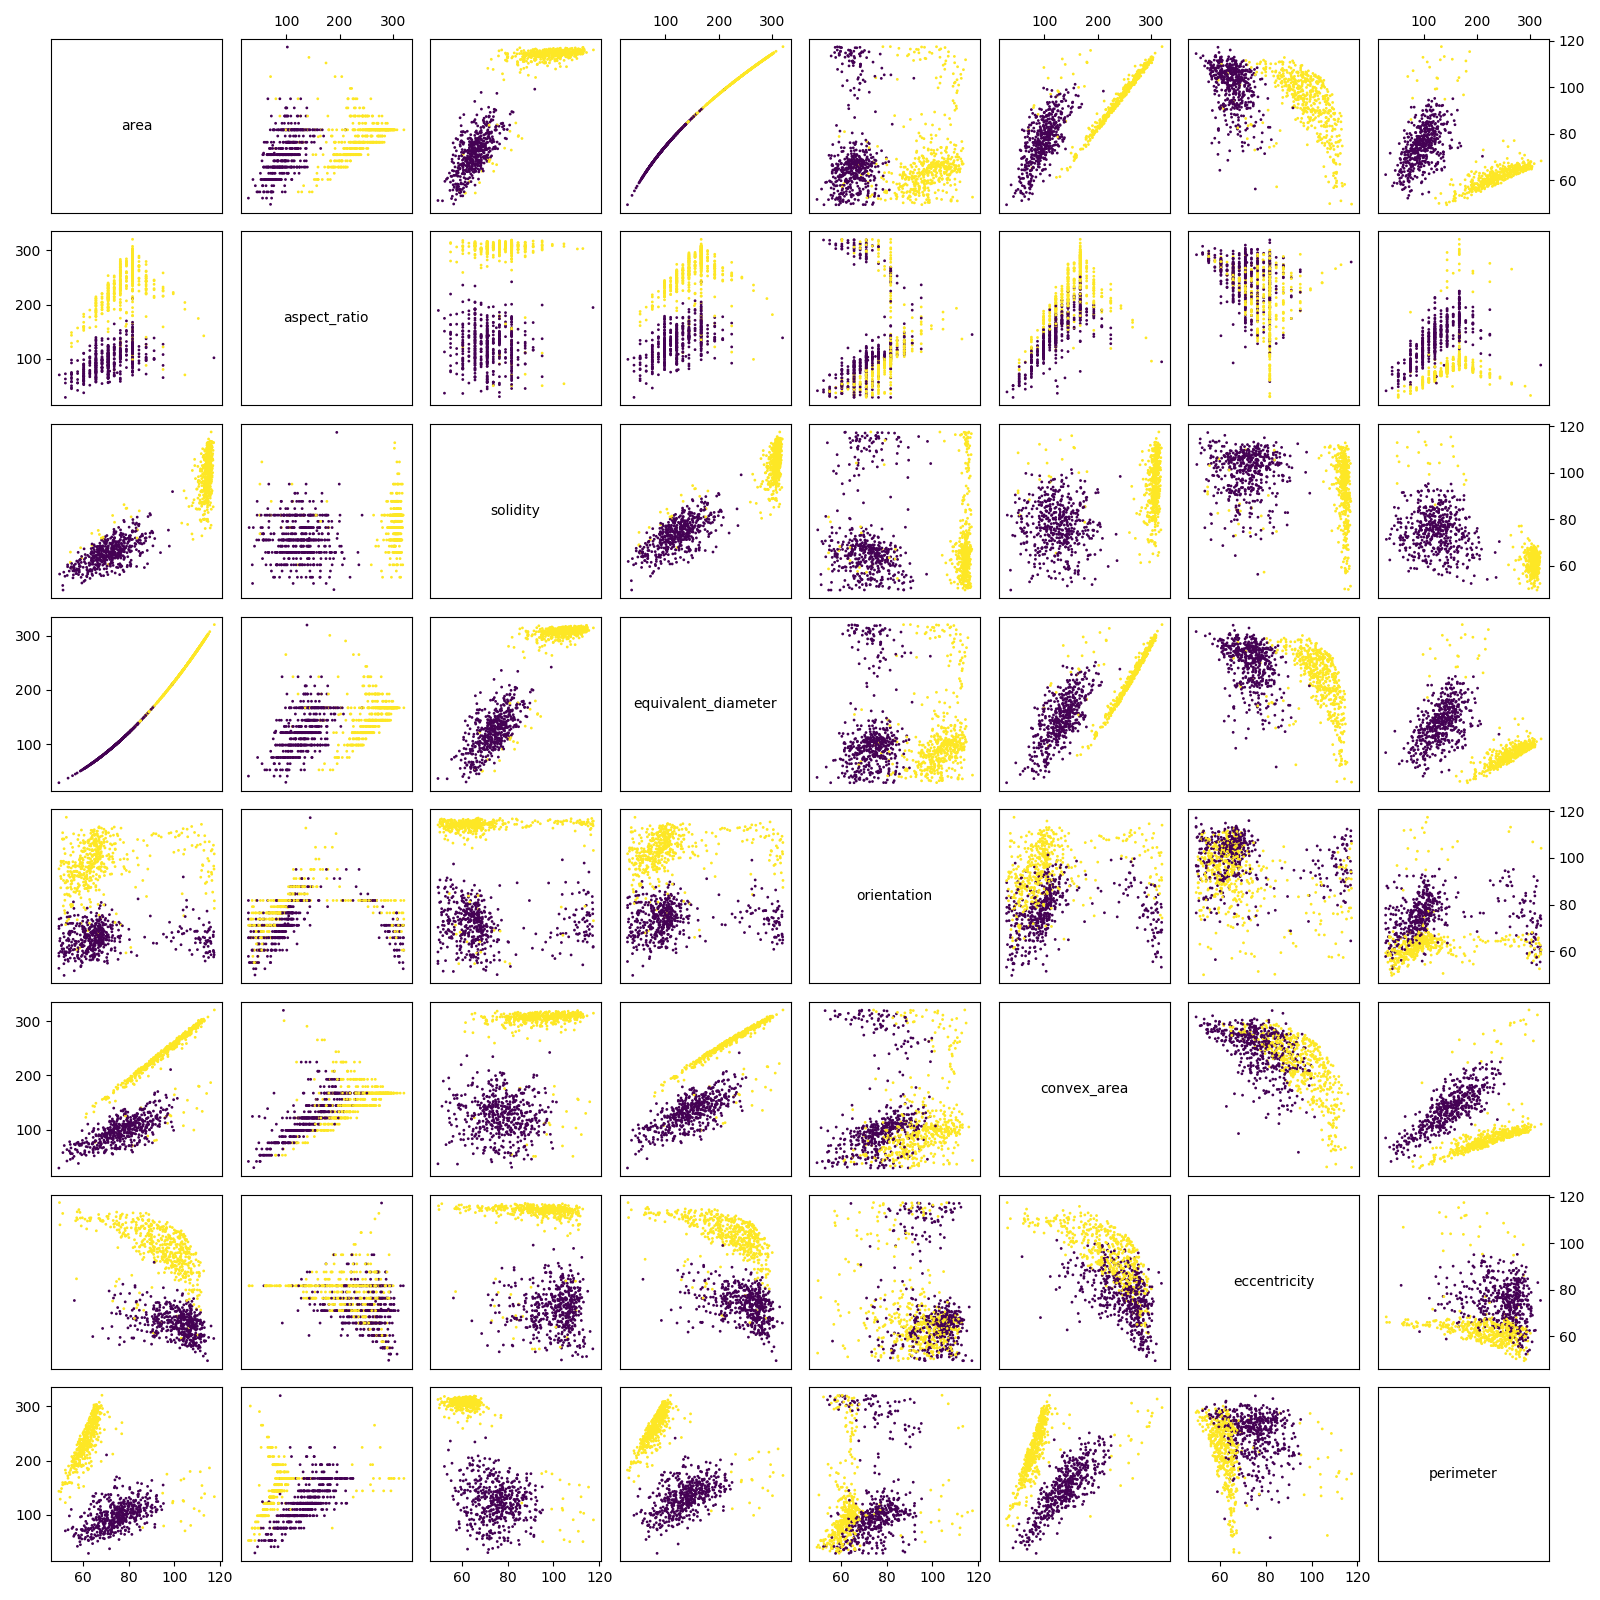
\includegraphics[width=\textwidth]{figures/scatter_matrix}
\caption{Scatter plot matrix of all region properties}
\label{perceptron:features}
\end{figure}

\subsubsection{Features without transform}

We used once the batch training algorithm and once the online training algorithm to classify the data directly from these to features. The connfusion matrix evaluated on a separate test set gives us following perfomance:

For the online training algorithm evaluated on the test set we got 385 correctly classified results of 400 test images. We got the following confusion matrix:

\begin{tabular}{ l | c | r }
\centering
  n=400 & classified as 1 & classified as 7 \\ \hline
  Digit 0 & 185 & 15 \\
  Digit 7 & 0 & 200 \\
\end{tabular}

For the batch training algorithm evaluated on the same test set we got 383 correctly classified results of 400 test images. We got the following confusion matrix:

\begin{tabular}{ l | c | r }
\centering
  n=400 & classified as 1 & classified as 7 \\ \hline
  Digit 0 & 187 & 13 \\
  Digit 7 & 4 & 200 \\
\end{tabular}

The corresponding decision boundries are shown in figure \ref{perceptron:decision:simple}. We see that the data is not linearly seperable, because there are yellow points inside the purple "cloud".

 In theory a perceptron is able to detect a linearly seperable set, because if the set is linearly seperable, then the algorithm is guaranteed to converge. Moreover we can bound the number of training steps from above. But as this bound depends on a separating hyperplane and the training set, we can not know beforehand how big this upper bound is.

\begin{figure}
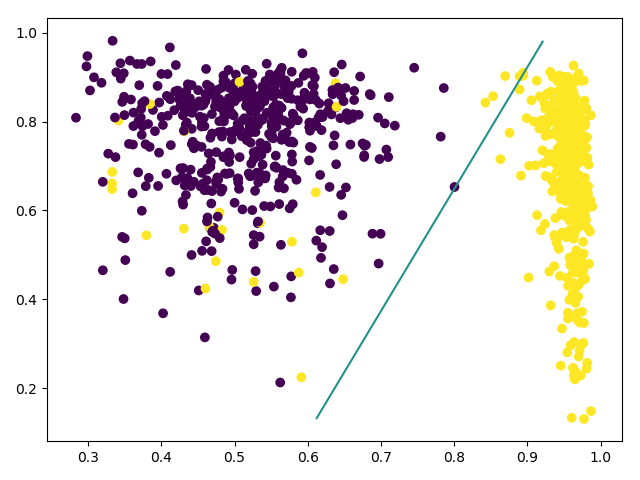
\includegraphics[width = 0.5\textwidth]{figures/decision_simple_online}
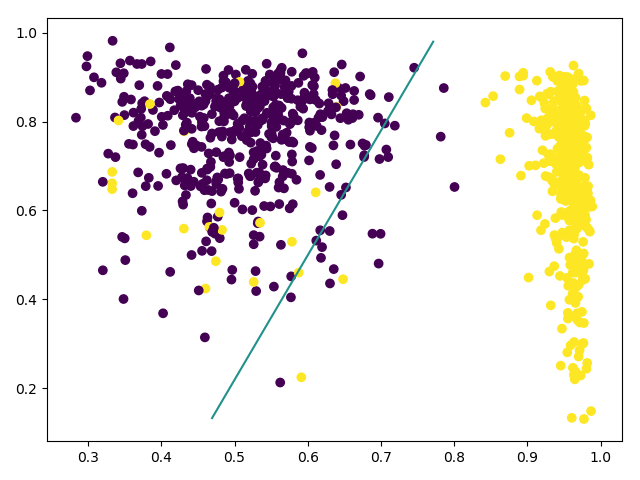
\includegraphics[width = 0.5\textwidth]{figures/decision_simple_batch}
\caption{The decision boundry of the trained perceptron. On the left for the online algorithm on the right for the batch algorithm.}
\label{perceptron:decision:simple}
\end{figure}

\subsubsection{Classification with feature transform}
We performed the same experiments as above, but first applied following feature transform to our data. $(x,y)\mapsto (1,x,y,x^2,y^2,xy)$

For the online training algorithm evaluated on the test set we got 386 correctly classified results of 400 test images. We got the following confusion matrix:

\begin{tabular}{ l | c | r }
\centering
  n=400 & classified as 1 & classified as 7 \\ \hline
  Digit 0 & 186 & 14 \\
  Digit 7 & 0 & 200 \\
\end{tabular}

For the batch training algorithm evaluated on the same test set we got 383 correctly classified results of 400 test images. We got the following confusion matrix:

\begin{tabular}{ l | c | r }
\centering
  n=400 & classified as 1 & classified as 7 \\ \hline
  Digit 0 & 187 & 13 \\
  Digit 7 & 4 & 200 \\
\end{tabular}

The corresponding decision boundries are shown in figure \ref{perceptron:decision:5d}. It's not very surprising that the feature transform doesn't help the classification. as there are yellow points, correspondig to the digit 0, inbetween purple points. Such a simple feature transform cannot separete this points, as the new decision boundry is just a quadratic.

\begin{figure}
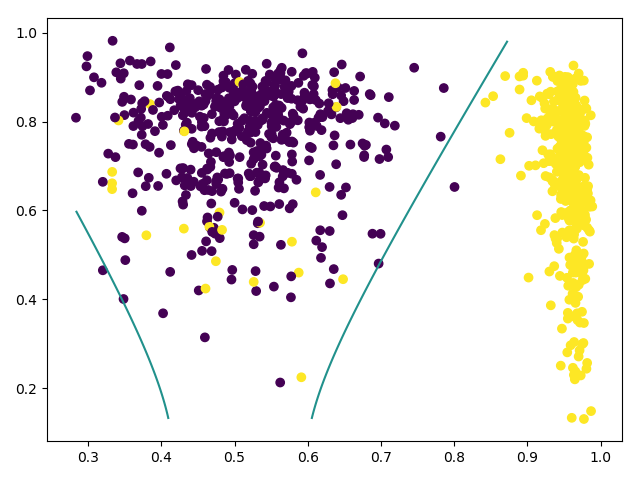
\includegraphics[width = 0.5\textwidth]{figures/decision_5d_online}
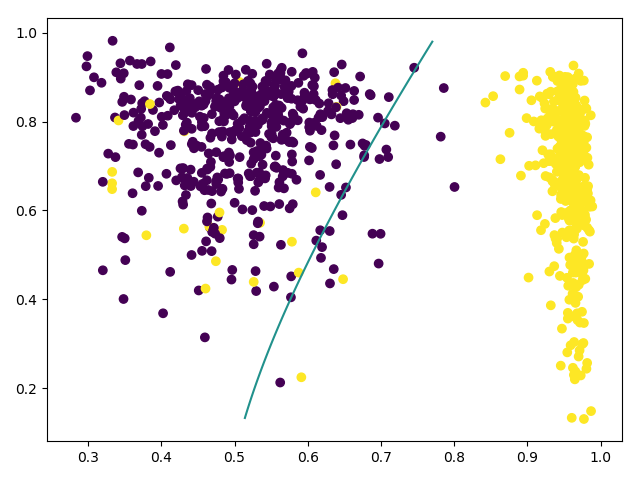
\includegraphics[width = 0.5\textwidth]{figures/decision_5d_batch}
\caption{The decision boundry of the trained perceptron. On the left for the online algorithm on the right for the batch algorithm.}
\label{perceptron:decision:5d}
\end{figure}

\subsubsection{Classification directly with image data}
We then tested the perceptron algorithm by using the image data as direct input. This is done by vectorizing the image into one vector. Instead of showing the corresponding decision boundry, we will visualize the calculated weight vector of the perceptron this is shown in figure \ref{perceptron:weights} for both the online and the batch algorithm.

We see that the weights resemble a bright 0 overlayed over a dark 7. This follows from the fact, that the perceptron tries to give images resembling a 7 a positive value and images resembling a 0 a negative value. We can also see that this is much clearer in the batch algorithm. We think this follows from the fact, that in the online algorithm the last data point observed has a big influence on the resulting weight vectors. On the other hand, as we compare a weight vector over the whole data set in the batch algorithm, each singular data point has much less relative influence on the resulting weights.

Moreover, in these experiment the training set was linearly seperable. And we got very good results on the test set, where the online algorithm even classified all images correctly. 

\begin{figure}
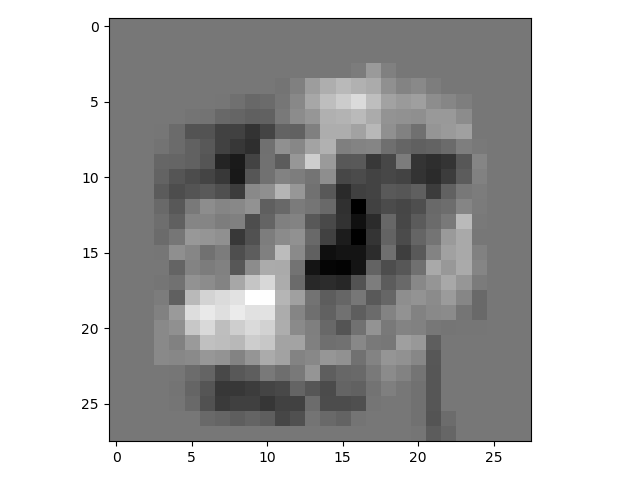
\includegraphics[width = 0.5\textwidth]{figures/weights_image_online}
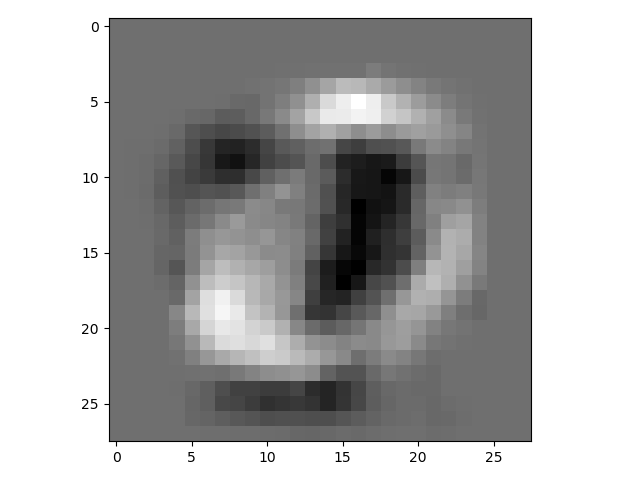
\includegraphics[width = 0.5\textwidth]{figures/weights_image_batch}
\caption{On the decision boundry of the trained perceptron. On the left for the online algorithm on the right for the batch algorithm.}
\label{perceptron:decision:5d}
\end{figure}

For the online training algorithm evaluated on the test set we got 400 correctly classified results of 400 test images. We got the following confusion matrix:

\begin{tabular}{ l | c | r }
\centering
  n=400 & classified as 1 & classified as 7 \\ \hline
  Digit 0 & 200 & 0 \\
  Digit 7 & 0 & 200 \\
\end{tabular}

For the batch training algorithm evaluated on the same test set we got 398 correctly classified results of 400 test images. We got the following confusion matrix:

\begin{tabular}{ l | c | r }
\centering
  n=400 & classified as 1 & classified as 7 \\ \hline
  Digit 0 & 200 & 0 \\
  Digit 7 & 2 & 198 \\
\end{tabular}

\subsection{Performance}
In the following table we summerize the performance of each experiment. We only report theerror rate, i.e. ratio of wrongly classified images, because the confusion matrices are already given above. We evaluated the perceptrons on a test set with 200 images of each class.


\begin{tabular}{ l | c | r }
\centering
  Experiment & Online error rate & Batch error rate \\ \hline
  2d features & 0.0375 & 0.0425 \\
  5d features & 0.035 & 0.0425 \\
  whole Images  & 0 & 0.005 \\
\end{tabular}


